\documentclass[11pt]{scrartcl}
\usepackage{wrapfig}
\usepackage{verbatim} 
\usepackage{acronym}
\usepackage[T1]{fontenc} % Use 8-bit encoding that has 256 glyphs
\usepackage{fourier} % Use the Adobe Utopia font for the document - comment this line to return to the LaTeX default
%\usepackage[english]{babel} % german headers
\usepackage{ucs}             % neccessary for äöü
\usepackage[utf8x]{inputenc} % utf8 support
\usepackage{amsmath,amsfonts,amsthm} % Math packages
\usepackage{hyperref}   % use for hypertext links, including those to external documents and URLs
\usepackage{enumitem}
\usepackage{float}
\usepackage{extramarks} % Required for headers and footers
\usepackage{graphicx} % Required to insert images
\usepackage{subfigure} % Required to insert images
\usepackage{listings} % Required for insertion of code
\usepackage{courier} % Required for the courier font
\usepackage{color}
\usepackage{sectsty} % Allows customizing section commands
\usepackage{epstopdf}
\usepackage[pass]{geometry}
\usepackage{cite}
\usepackage{textcomp}
\usepackage{subfiles}
% Style of citations
\bibliographystyle{plain}  
\usepackage{./sty/fhv}

%language
\usepackage[ngerman]{babel}

%general data
\newcommand{\myauthor}{Nicolaj Höss, Marko Petrovi\'c, Kevin Wallis}
\newcommand{\mytitle}{Embedded Betriebssystem}
\newcommand{\mysubtitle}{für ARM Cortex-A8}
\newcommand{\myuniversity}{Fachhochschule Vorarlberg}
\newcommand{\mycourse}{S1: Softwarelösungen für ressourcenbeschränkte Systeme}
\newcommand{\mystudy}{Master Informatik (ITM2)}
\newcommand{\mydate}{\today{}, Dornbirn}
%document meta data
\title{\mytitle}
\author{\myauthor}
\date{\today{}, Dornbirn}

%header/footer - KOMA
\usepackage{lastpage}
\usepackage[automark]{scrpage2}
\pagestyle{scrheadings}
\clearscrheadfoot
%header left
\ihead[]{\headmark}
%header center
\chead[]{}
%header right
\ohead[]{
\includegraphics[width=2cm]{figures/FHV} }
%footer left
\ifoot[]{\myauthor}
%footer center
\cfoot[]{}
%footer right
\ofoot[]{\thepage\ von \pageref{LastPage}}

\usepackage{color}				% defining syntax colours
\definecolor{mygreen}{rgb}{0,0.6,0}
\definecolor{mygray}{rgb}{0.5,0.5,0.5}
\definecolor{mymauve}{rgb}{0.58,0,0.82}

\lstset{ 
  language=Matlab, 
  backgroundcolor=\color{white},
  numbers=left,
  numbersep=5pt,
  showstringspaces=false,
  frame=single,
  rulecolor=\color{black},
  showspaces=false,
  showstringspaces=false,
  showtabs=false,
  tabsize=2,
  breaklines=true,
  captionpos=tl,
  basicstyle=\footnotesize,
  commentstyle=\color{mygreen},
  keywordstyle=\color{blue},     
  stringstyle=\color{mymauve},
  postbreak=\raisebox{0ex}[0ex][0ex]{\ensuremath{\color{red}\hookrightarrow\space}}}


\begin{document}

%%Titelseite
\begin{titlepage}

\begin{minipage}{.5\textwidth} 
  \hspace{12cm}\hfill 
\includegraphics[width=3cm]{figures/FHV} 
\end{minipage}\vspace{2cm} 

\begin{center}
~
\vfill\vfill\vfill

{\Huge\bfseries\mytitle} \\
{\Large\bfseries\mysubtitle}

\vfill

\Large{eine Arbeit von}

\vfill

{\LARGE\bfseries\myauthor}
\vfill
{\Large\bfseries\mystudy}
\vfill
\vfill
\Large{für die Lehrveranstaltung}

\vfill

{\LARGE\bfseries\mycourse}

\vfill\vfill\vfill
\vfill\vfill\vfill
\vfill\vfill\vfill

\myuniversity
\vfill
\mydate
\end{center}
\end{titlepage}
%%Ende Titelseite

%%Abstract
\begin{abstract}
\thispagestyle{plain}
	
\section*{Abstract}

\end{abstract}

\thispagestyle{plain}
%%Inhaltsverzeichnis
\tableofcontents

\newpage
%%Abbildungsverzeichnis
\listoffigures
\newpage
\pagebreak

\section*{Abkürzungsverzeichnis}

\vspace{1cm}
\begin{acronym}[Bash]
	\acro{AINTC}{ARM Interrupt Controller}
	\acro{CWD}{Current Working Directory}
	\acro{DALI}{Digital Addressable Lighting Interface (Bus Protokoll)}
	\acro{DFAR}{Data Fault Address Register}
	\acro{DFSR}{Data Fault Status Register}
	\acro{DMX}{Digital Multiplex (Bus Protokoll)}
	\acro{GPIO}{General Purpose Input Output}
	\acro{UART}{Universal Asynchronous Receiver Transmitter}
	\acro{HAL}{Hardware Abstraction Layer}
	\acro{KNX}{Konnex-Bus (Bus Protokoll)}
	\acro{MMU}{Memory Management Unit}
	\acro{MPT}{Master Page Table}
	\acro{OS}{Operating System}
	\acro{PTE}{Page Table Entry}
	\acro{LPAE}{Large Physical Address Extension}
	\acro{SCTLR}{System Control Register}
	\acro{TLB}{Translation Lookaside Buffer}
	\acro{TTBCR}{Translation Table Base Control Register}
	\acro{TTBR}{Translation Table Base Register}
	\acro{VMSAv7}{Virtual Memory System Architecture for ARMv7}
\end{acronym}

\pagebreak 
\section{Allgemein}
bla

\subsection{Aufbau}
bla

\pagebreak 
\section{Projektmanagement}
Im folgenden Abschnitt werden einige Punkte zum Projektmanagement erklärt. 

\subsection{Prozessmodell}
Als Prozessmodell wurde SCRUM mit einigen Abänderungen umgesetzt. Wobei das zentrale Vorgehen in Bezug auf Agilität bestmöglich übernommen wurde. Gründe für die Verwendung von SCRUM:

\begin{itemize}
	\item Agilität
	\item Nach jedem Sprint ein lauffähiges System
	\item Klares Ziel für jeden Sprint
	\item Einfaches Hinzufügen fehlender Aufgaben (neue Stories)
	\item Einfaches neu priorisieren von Aufgaben
	\item Ereignisse die den Entwicklungszyklus beeinflussen (z.B. Klausuren) beeinträchtigen das weitere Vorgehen nicht
	\item Klare Übersicht der fehlenden Stories
\end{itemize}

\subsection{Versionsverwaltung}
Als Versionsverwaltung wurde Git verwendet. Zwei Gründe für die Verwendung von Git sind leichte Einbindung im Zusammenhang mit dem Repository (siehe \ref{Repository}) und die Möglichkeit der Nicht-linearen Entwicklung.

\subsection{Repository}
Github.

\pagebreak 
\section{Architektur}
\label{chapArch}
Dieses Kapitel beschreibt die entwickelte Architektur des Betriebssystems und gibt einen groben Überblick über die einzelnen Komponenten. Detailliertere Informationen zu den einzelnen Komponenten werden in den folgenden Kapiteln beschrieben.

\subsection{Art des Kernels}
Das Betriebssystem wurde als Monolithischer Kernel umgesetzt, respektive wurden die Speicherverwaltung, Prozessverwaltung, Treiber und andere Kernelkomponenten in einem einzelnen Kernelprozess implementiert. Durch die Zusammenführung dieser Komponenten verliert das Betriebssystem zwar die Eigenschaft, nach einem Absturz einer einzelnen Komponente weiter lauffähig zu sein, allerdings darf mit diesem Konzept durchaus von einer höheren Performanz ausgegangen werden.
Ein weiterer Grund für einen Monolithischen Kernel ist das entfallen der aufwändigen Kommunikationen zwischen den verschiedenen Komponenten des Betriebssystems, welche besonders in der Anfangsphase der Entwicklungsarbeiten zu Problemen führen kann.

\subsection{Ansatz für die Abstraktionen im Betriebssystem}
Um eine möglichst gute Abstraktionen der Betriebssystem-Implementierung zu gewährleisten, wurden für die Verwaltung einzelner Kernelkomponenten \textit{Manager} verwendet. Im Allgemeinen gilt, dass die einzelnen \textit{Manager} jeweils die Schnittstelle für eine Komponente darstellen. Die Kommunikation zwischen zwei Komponenten erfolgt ausschließlich über die bereitgestellte Schnittstelle des \textit{Managers}. Eine Übersicht der einzelnen \textit{Manager} sowie eine bzw. mehrere zugehörige Funktionen, ist in Tabelle \ref{table:Manager-function} angegeben.

\begin{table}[H]
\begin{tabular}{p{4cm} | p{9cm}}
  \textbf{Managername} & \textbf{Beispiel Funktion(en)} \\ 
  \hline
  \textit{DeviceManager} & \texttt{InitDevice}, \texttt{OpenDevice}, \texttt{ReadDevice} \\
  \textit{DriverManager} & \texttt{GetDriver} \\
  \textit{FileManager} & \texttt{OpenFile}, \texttt{OpenExecutable} \\
  \textit{MemManager} & \texttt{GetFreePagesInProcessRegion}, \texttt{GetRegion} \\
  \textit{ProcessManager} & \texttt{StartProcess}, \texttt{KillProcess} \\
  \textit{IpcManager} & \texttt{RegisterNamespace}, \texttt{SendMessage} \\
 \end{tabular}
 \caption{Übersicht der Manager mit beispielhaften Funktionen}
 \label{table:Manager-function}
\end{table}

\subsection{Allgemeiner Aufbau der Architektur}
\label{section:generalArchitecture}
In Abbildung \ref{fig:general-Architecture} ist der allgemeine Aufbau mit den wesentlichen Kernelkomponenten ersichtlich. Zusätzlich zu den einzelnen Komponenten ist ebenfalls der Informationsfluss dargestellt.

\begin{figure}[H]
	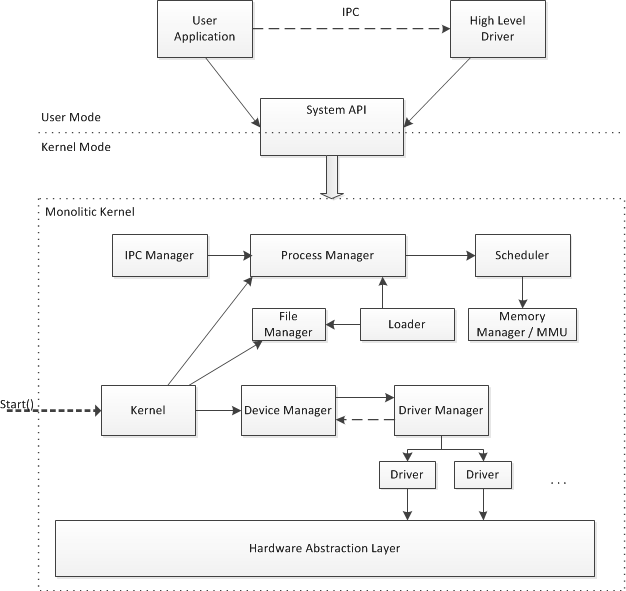
\includegraphics[scale=0.9]{chapters/architecture/figures/architecture}
	\caption{Allgemeiner Aufbau der Architektur}
	\label{fig:general-Architecture}
\end{figure}

Die oben angeführten Komponenten und deren Verantwortlichkeiten sind im Folgenden grob beschrieben: \\

\begin{description}
	\item[Hardware Abstraction Layer (HAL)] \hfill \\
	Der \ac{HAL} abstrahiert sämtlichen Hardwarezugriff des Betriebssystems und erlaubt so eine einfache Portierbarkeit auf andere Plattformen. Der Aufbau des \ac{HAL} wird in Kapitel \ref{chapHAL} beschrieben.
	
	\item[Driver] \hfill \\
	Ein Treiber bietet eine abstrakte Schnittstelle zur jeweiligen Hardware, respektive implementiert dieser die konkrete Ansteuerung. Der Aufbau der Treiber ist in Kapitel \ref{chapDriver} dokumentiert. 
	
	\item[\textit{DriverManager}] \hfill \\
	Der \textit{DriverManager} dient zur Verwaltung der Treiber, welche vom Betriebssystem zur Verfügung gestellt werden. Sollte ein Treiber benötigt werden, kann über die Schnittstelle des \textit{DriverManagers} der Zugriff auf den Treiber erfolgen. Der detaillierte Aufbau des \textit{DriverManager} ist in Kapitel \ref{secDriverManager} erläutert.
	
	\item[\textit{DeviceManager}] \hfill \\
	Der \textit{DeviceManager} ist eine weitere Abstraktion zur Verwaltung von Treibern, respektive einzelnen Geräten. So sind beispielsweise auf Treiberebene alle vier Board-LEDs als identisch anzusehen, allerdings stellen sie auf Geräteebene jeweils vier unterschiedliche Geräte dar, welche aber vom selben Treiber angesprochen werden können. In Kapitel \ref{secDeviceManager} wird die Verantwortlichkeit des \textit{DeviceManagers} genauer diskutiert.
	
	\item[Kernel] \hfill \\
	Der Kernel weist die Verantwortlichkeit für das Starten der einzelnen Komponenten auf und stellt grundlegende Funktionsschnittstellen für die einzelnen Komponenten zur Verfügung. Beispielsweise werden sämtliche Fehler oder Ausgaben von Kernelkomponenten an den Kernel selbst propagiert.
	
	\item[\textit{ProcessManager}] \hfill \\
	Der \textit{ProcessManager} stellt eine Schnittstelle für den Zugriff auf Prozesse zur Verfügung. Weiters verwaltet der \textit{ProcessManager} Meta-Daten zu den einzelnen Prozessen, wie Prozessname, Startzeit usw. Implementierungsdetails zum \textit{ProcessManager} werden in Kapitel \ref{secProcessManager} beschrieben.
	
	\item[\textit{Scheduler}] \hfill \\
	Der \textit{Scheduler} verwaltet die Prozesse auf einer abstrakten Ebene, respektive hinsichtlich ihrer Zustände, ihres Kontexts usw. Weiters ist der \textit{Scheduler}für die Umsetzung des präemptiven Multi-Taskings verantwortlich. Die konkrete Implementierung ist in Kapitel \ref{secScheduler} beschrieben.
	
	\item[\textit{MemoryManager}/\ac{MMU}] \hfill \\
	Der \textit{MemoryManager} stellt die Schnittstelle zum virtuellen Speichermanagement zur Verfügung. Diese Komponente übernimmt ebenfalls die Verwantwortlichkeit für die Verwaltung des virtuellen und physischen Speichers. Der \textit{MemoryManager} bzw. das Speichermanagement im Allgemeinen ist im Kapitel \ref{chapVirtualMemory} beschrieben.

	\item[\textit{FileManager}] \hfill \\
	Der \textit{FileManager} stellt die Schnittstelle zum Zugriff auf das Dateisystem, respektive Dateien und Ordner zur Verfügung. Der \textit{FileManager} verwaltet ebenfalls die \ac{CWD} des Benutzers bzw. der Benutzerin.
	
	\item[\textit{Loader}] \hfill \\
	Der \textit{Loader} ist für das Laden von Anwendungen verantwortlich, respektive lädt der \textit{Loader} eine Anwendung von einem externen Speichermedium in den Arbeitsspeicher, sodass dieser als Prozess ausgeführt werden kann.
	
	\item[\textit{IPCManager}] \hfill \\
	Der \textit{IPCManager} ist für die Kommunikation zwischen verschiedenen User-Anwendungen zuständig. Die Dokumentation der Interprozesskommunikation ist in Kapitel \ref{chapIPC} festgehalten.
	
	\item[System-API] \hfill \\
	Die System-API stellt eine Schnittstelle zum Betriebssystem für Anwendungen zur Verfügung. Hierdurch sind die Betriebssystemfunktionen von der Anwendung selbst entkoppelt. Dies erlaubt einen sicheren Zugriff auf Geräte und Ressourcen. Die System-API ist in Kapitel \ref{chapAPI} beschrieben.
	
	\item[\textit{User Application}] \hfill \\
	\textit{User Applications} (dt. Anwendung) sind Prozesse welche von einem externen Speichermedium geladen werden. Diese können mittels Interprozesskommunikation mit anderen Anwendungen oder mittels der System-API mit anderen Komponenten kommunizieren. Im Kapitel \ref{chapApp} ist eine konkrete Implementierung einer Anwendung dokumentiert.
	
	\item[\textit{High Level Driver}] \hfill \\
	\textit{High Level Driver} sind Treiber, welche einer Anwendung eine breitere Schnittstelle als Kernel-interne Treiber anbieten und unter anderem auch erweiterte Funktionen implementieren. Beispielswiese wird durch den \textit{High Level Driver} für das Ansteuern eines \textit{Moving Heads} über das \ac{DMX}-Protokoll das zyklische Senden des aktuellen Zustands realisiert. 
\end{description}

\pagebreak 
\section{HAL}
bla

\subsection{Aufbau}
bla

\pagebreak 
\section{Treiber}
Die Treiber stellen eine abstrakte Schnittstelle auf den Hardware Abstraction Layer dar. Dadurch muss nicht mehr direkt auf die einzelnen Hardwarekomponenten zugegriffen werden. Ein wesentlicher Aspekt bei der Architektur der Treiber war Abstraktion. Dadurch wird gewährleistet, dass jeder Treiber über die selbe Schnittstelle angesprochen werden kann. Zudem ist die Verwaltung durch den Driver Manager erleichtert.

\subsection{Aufbau eines Treibers}
In Listening \ref{generalDriverInterface} ist die allgemeine Schnittstelle für jeden Treiber ersichtlich. Jeder implementierte Treiber muss diese vorweisen können, ein Beispiel (LED Treiber) dazu ist in Listening \ref{ledDriver} zu sehen.

\lstinputlisting[language=C, caption=Allgemeine Schnittstelle für einen Treiber, label=generalDriverInterface]{chapters/driver/codefiles/generalDriverInterface.c}

\lstinputlisting[language=C, caption=Implementierung der allgemeinen Treiberschnittstelle (LED Beispiel), label=ledDriver]{chapters/driver/codefiles/ledDriver.c}


\pagebreak 
\section{Prozessverwaltung}
Als Prozessverwaltung wird hauptsächlich das Verwalten von Prozessen durch das Betriebssystem verstanden (Vgl. http://www.lowlevel.eu/wiki/Prozessverwaltung). Jeder Prozess besitzt eine eindeutige Identifikation (PID), durch welche dieser vom System angesprochen werden kann. 

\subsection{Prozesszustände}
Jeder Prozess besitzt zu einem bestimmten Zeitpunkt einen fix definierten Zustand, d.h. es können keine Inkonsistenzen auftreten. Abbildung \ref{fig:Process-states} zeigt die verschiedenen Zustände eines Prozesses sowie die jeweilig erlaubten Übergänge zu einem anderen Zustand auf.

\begin{figure}[H]
	
\includegraphics[scale=0.60]{chapters/processmanagement/figures/todo}
	\caption{Erlaubte Prozesszustände und Prozessübergänge}
	\label{fig:Process-states}
\end{figure}

Im folgenden wird eine detaillierte Erklärung zu den einzelnen Zuständen aus Abbildung \ref{fig:Process-states} gegeben.

\begin{description}
	\item[Ready] \hfill \\
	Der Zustand ready tritt ein, wenn ein Prozess bereit wäre um ausgeführt zu werden. 
	
	\item[Running] \hfill \\
	Ein Prozess weist diesen Zustand auf, wenn er gerade ausgeführt wird. Es gibt immer nur einen running Prozess zu einem bestimmten Zeitpunkt.
	
	\item[Blocked] \hfill \\
	XXX
	
	\item[Sleeping] \hfill \\
	XXX	
	
	\item[Free] \hfill \\
	XXX
\end{description}

Es gibt unterschiedliche Zustandsübergänge, welche im Betriebssystem erlaubt sind. Tabelle \ref{table:State-transition} stellt die verschiedenen Übergänge mit einem dazu passenden Beispiel dar.

\begin{table}[H]
\begin{tabular}{p{3cm} | p{3cm} | p{6cm}}
  \textbf{Ausgangszustand} & \textbf{Nächster Zustand} & \textbf{Beispiel} 
  \\ \hline
  Ready & Running & XXX \\
  Running & Blocked & XXX \\
  Running & XXX & XXX \\
  XXX & XXX & XXX \\
  
 \end{tabular}
 \caption{Erlaubte Zustandsübergänge mit Beispiel}
 \label{table:State-transition}
\end{table}


\begin{figure}[H]
	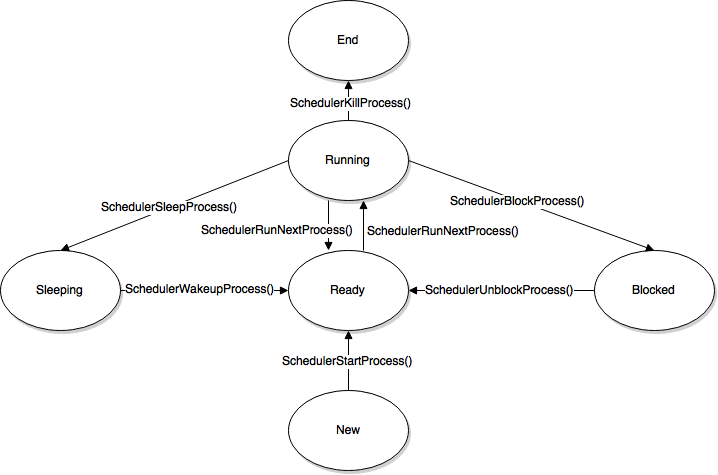
\includegraphics[scale=0.60]{chapters/processmanagement/figures/StateTransition}
	\caption{Prozesszustände und deren Transitionen}
	\label{fig:StateTransition}
\end{figure}

\subsection{Scheduler Eigenschaften}
Der Scheduler weißt eine Zeitscheibe von $10ms$ auf, d.h. jeder Prozess hat $10ms$ bevor er gewechselt wird. Sollte ein anderer Prozess zur Verfügung stehen wird dieser genommen ansonsten bekommt der gleicher Prozesse erneut eine Zeitscheibe von $10ms$. Diese Zeitscheibendauer wurde aufgrund mehrerer Aspekte gewählt: eine zu große Zeitscheibe $>$ $100ms$ würde merkbaren Verzögerungen im Betriebssystem führen, bei einer zu kleinen Zeitscheibe $<$ $1ms$ würde die benötigte Zeit für einen Wechsel im Vergleich zu lange dauern. Durchgeführte Performanztests sind im Kapitel XXX aufgeführt. \\ \\
Das verwendete Schedulingverfahren ist Round Robin. Bei der Verwendung eines Verfahrens mit Prioritäten hätte der Fall mit einem hoch priorisierten Prozesse beachtet werden müssen. Ein Beispiel dazu: Es gibt drei Prioritäten (hoch, mittel und niedrig). Die Konsole wird als hoch eingestuft alle anderen Prozesse sind niedriger priorisiert. Wie bekommt nun ein mittel/niedrig priorisierter Prozess eine Zeitscheibe?

\subsection{Vorgehen bei der Prozessverwaltung}
Das Vorgehen bei der Prozessverwaltung wird im Sequenzdiagramm von Figure \ref{Sequencediagram} dargestellt. Ein Client übergibt dem ProcessManager die Aufgabe einen Prozess zu erzeugen. Dieser delegiert das Erzeugen des Prozesses an den Scheduler weiter. Hierbei ist zu beachten, dass die Metadaten vom Prozess nicht weitergegeben werden. Der Scheduler speichert sich diesen neuen Prozess in seiner Prozesstabelle ab. Das MemoryManagement dient zum Allokieren von benötigtem Speicherplatz für den neuen Prozess. Der erzeugte Prozess wird an den ProcessManager zurückgegeben, wobei dieser noch MetaInformationen beifügt (z.B. den Namen des Prozesses). Dem Client wird am Ende mitgeteilt, ob das Erzeugen erfolgreich war. Ein alternativer Rückgabeparameter wäre die PID, wobei hier darauf zu achten ist, dass im Fehlerfall eine ungültige PID zurückgeliefert wird.

\begin{figure}[H]
	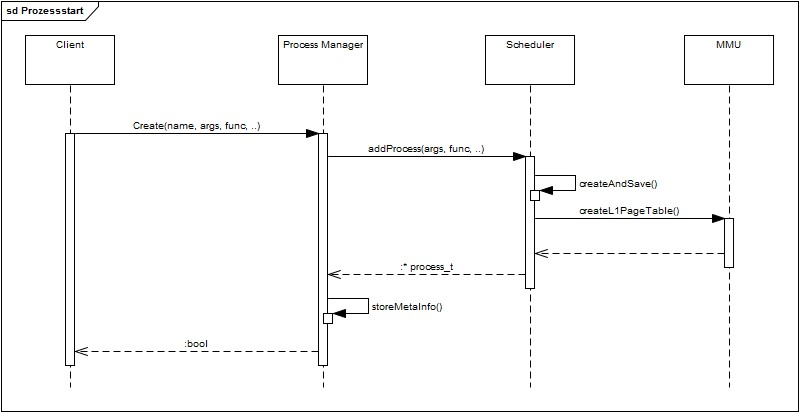
\includegraphics[scale=0.70]{chapters/processmanagement/figures/processmanagement-sequence-diagram}
	\caption{Sequenzdiagramm der Prozessverwaltung}
	\label{fig:Sequencediagram}
\end{figure}

\pagebreak 
\section{Virtuelle Speicherverwaltung}
\label{chapVirtualMemory}
Bei der virtuellen Speicherverwaltung erfolgt die Umwandlung von vom ARM Prozessor generierten, virtuellen Adressen in physikalische Adressen durch die \ac{MMU}. Dieses Kapitel enthält die Beschreibung des Designs und der Implementierung der virtuellen Speicherverwaltung des Betriebssystems sowie der Einstellungen der MMU.\\

\subsection{Grundlegende Funktionsweise}

Die \ac{VMSAv7} definiert zwei unabhängige Formate für translation tables \cite[S. B3-1318]{ARM:ARM}:

\begin{itemize}
	\item \emph{Short-descriptor format}:
	\begin{itemize}
		\item zweistufige Seitentabelle 
		\item 32-bit Deskriptoren (PTE)
		\item 32-bit virtuelle Eingangsadresse 
		\item bis zu 40-bit große physikalische Ausgangsadresse
	\end{itemize}
	\item \emph{Long-descriptor format}:
	\begin{itemize}
		\item dreistufige Seitentabelle
		\item 64-bit Deskriptoren (\acs{PTE})
		\item verwendet \emph{Large Physical Address Extension} (LPAE)
		\item bis zu 40-bit große virtuelle Eingangsadresse 
		\item bis zu 40-bit große physikalische Ausgangsadresse
	\end{itemize}
\end{itemize}

Um die Anforderungen an das Betriebssystem zu erfüllen, reicht das zweistufige Seitentabellensystem vollkommen aus. Tabelle \ref{table:GeneralVirtualMemory} fasst die wichtigsten gegebenen Eigenschaften unter Verwendung des Short-descriptor format zusammen.\\

\begin{table}[H]
\begin{tabular}{p{7cm} | p{7cm}}
  \textbf{Eigenschaft} & \textbf{Speicherbedarf} \\ \hline
  Virtueller Speicher & 4 GB\\  
  Größe eines Page Table Entry (PTE) & 4 Byte \\
  Einträge L1 Page Table & 4096\\
  Einträge L2 Page Table & 256\\
  Speicherbedarf L1 Page Table & 4 Byte * 4096 = 16kB \\
  Speicherbedarf L2 Page Table & 4 Byte * 256 = 1kB\\
  Unterstützte Pagegrößen: & \emph{small page} (4 kB), \emph{large page} (64 kB)\\
  Unterstützte Sectiongrößen: & \emph{section} (1 MB), \emph{supersection} (16 MB)\\
 \end{tabular}
 \caption{Eigenschaften der virtuellen Speicherverwaltung der ARMv7-Architektur}
 \label{table:GeneralVirtualMemory}
\end{table}

Generiert die ARM CPU einen Speicherzugriff, wird von der MMU ein Suchlauf durchgeführt. Dieser Suchlauf wird \emph{translation table lookup} genannt. Dabei wird zuerst im \ac{TLB} nachgesehen, ob einer der 64 Einträge des TLB die zur virtuellen Adresse korrespondierende physikalische Adresse enthält. Ist dies der Fall (so genannter \emph{TLB hit}), wird der Suchlauf an dieser Stelle erfolgreich beendet.\\

Ist die angeforderte virtuelle Adresse nicht im TLB enthalten (TLB miss), wird ein page table walk durchgeführt. Das Funktionsprinzip des zweistufigen Seitentabellensystems zeigt Abbildung \ref{fig:2levelTableSystem}. Aus einem der zwei Seitentabellenregister wird die Basisadresse der darin zuvor abgelegten L1-Seitentabelle geholt. Das Format der PTE bestimmt dann, um welchen Typ von Verweis es sich handelt. Seitentabellen und ihre Einträge werden im nachfolgenden Abschnitt \ref{subsect:pageTables} genauer beschrieben.\\

\begin{figure}[H]
	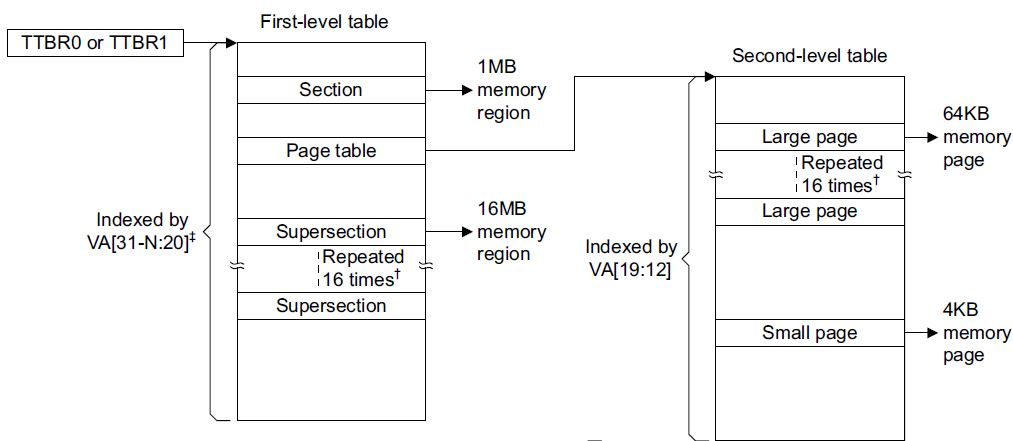
\includegraphics[scale=0.7]{chapters/mmu/figures/addressTranslation}
	\caption{Zweistufiges Seitentabellensystem \cite[S. B3-1325]{ARM:ARM}}
	\label{fig:2levelTableSystem}
\end{figure}


\subsection{Umwandlung virtueller Adressen zu physikalische Adressen}

Der genaue Vorgang der Umwandlung einer vom ARM Prozessor erzeugten virtuellen Adresse in eine physikalische Speicheradresse zeigen die nachfolgenden beiden Abbildungen. Abbildung  \ref{fig:sectionTranslation} zeigt die Umwandlung einer virtuellen Adresse in die physikalische Adresse einer 1 MB Section ohne Verwendung einer L2-Seitentabelle, Abbildung \ref{fig:smallPageTranslation} diejenige einer virtuellen Adresse in ein 4 kB page frame unter Verwendung einer L2-Seitentabelle.   Die Umwandlung wird vollständig durch die Prozessor-Hardware durchgeführt.\\


\begin{figure}[H]
	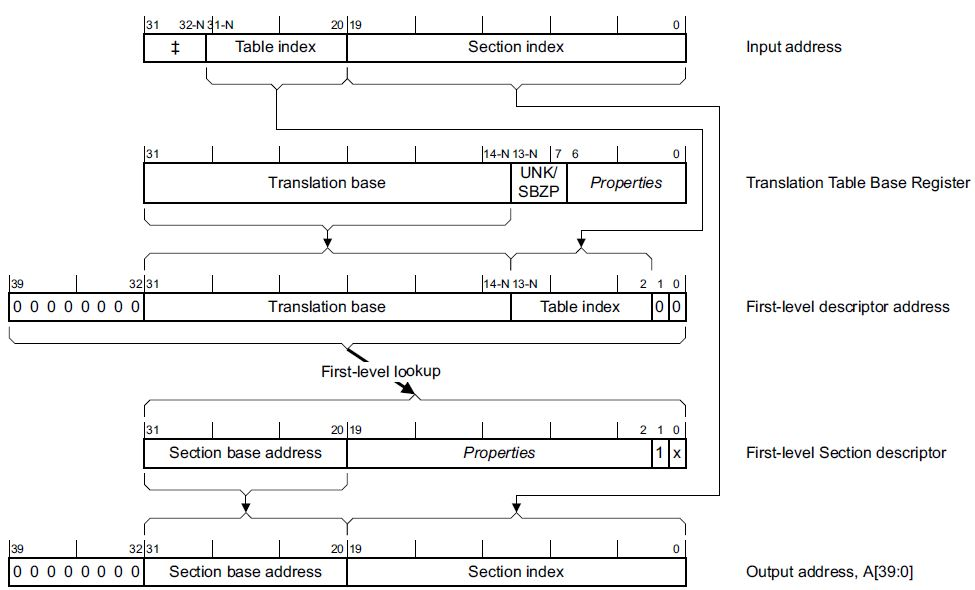
\includegraphics[scale=0.8]{chapters/mmu/figures/sectionTranslation}
	\caption{1 MB Section Translation durch die ARM CPU \cite[S. B3-1335]{ARM:ARM}}
	\label{fig:sectionTranslation}
\end{figure}

\begin{figure}[H]
	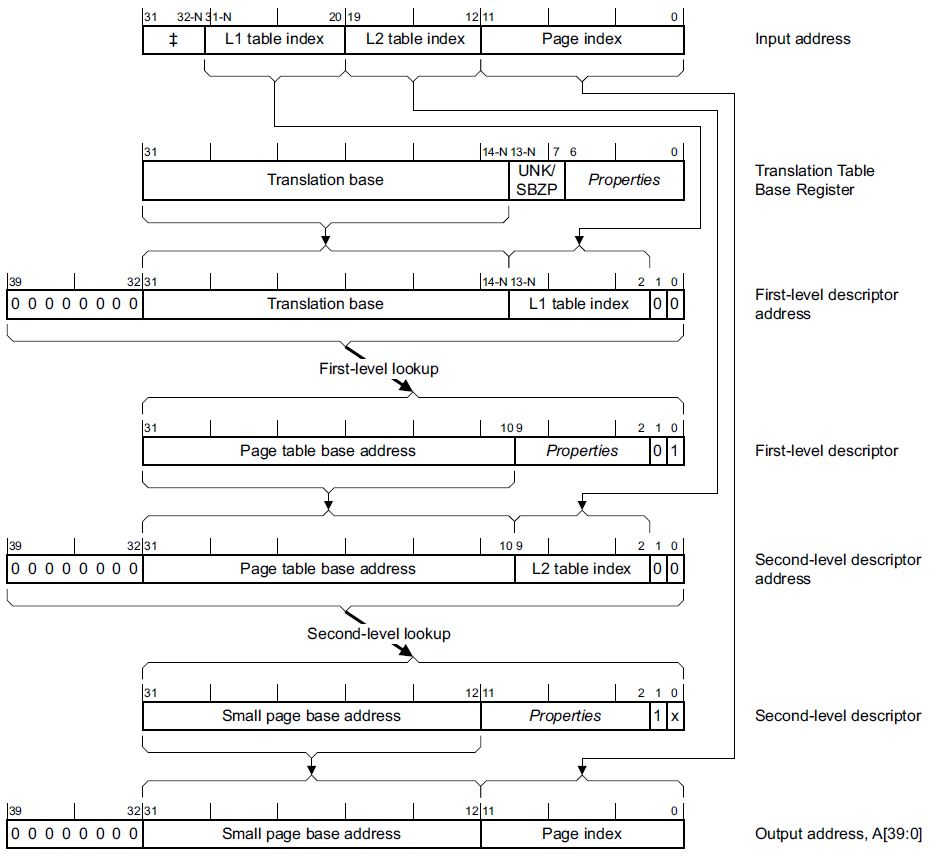
\includegraphics[scale=0.8]{chapters/mmu/figures/smallPageTranslation}
	\caption{Small Page Translation durch die ARM CPU \cite[S. B3-1337]{ARM:ARM}}
	\label{fig:smallPageTranslation}
\end{figure}

\subsection{Seitentabellen und Seitentabelleneinträge}
\label{subsect:pageTables}

Der verwendete ARM Prozessor verfügt über zwei Register (\acf{TTBR}, \emph{TTBR0} und \emph{TTBR1}), welche Startadressen von Seitentabellen enthalten  \cite[S. B3-1320]{ARM:ARM}. Ihre Formate sind nahezu identisch und in den Abbildungen \ref{fig:TTBR0Format} und \ref{fig:TTBR1Format} zu sehen. Diese Register übernehmen im Betriebssystem die folgende Funktion:

\begin{itemize}
	\item TTBR0: Wird für prozessspezifische Adressen verwendet. Jeder Prozess enthält bei seiner Initialisierung eine eigene L1-Seitentabelle. Bei einem Kontextwechsel erhält das TTBR0 eine Referenz auf L1-Seitentabelle des neuen Kontextes/Prozesses.
	\item TTBR1: Wird für das Betriebssystem selbst und für memory-mapped I/O verwendet. Diese ändern sich bei einem Kontextwechsel nicht.
\end{itemize}


\begin{figure}[H]
	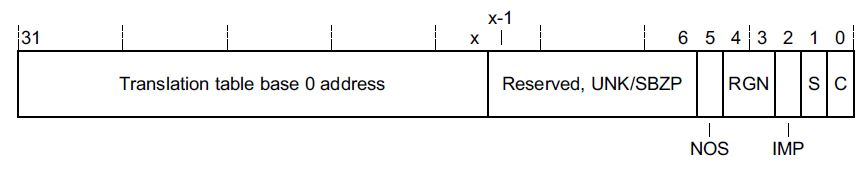
\includegraphics[scale=0.8]{chapters/mmu/figures/ttbr0format}
	\caption{TTBR0 Format \cite[S. B4-1726]{ARM:ARM}}
	\label{fig:TTBR0Format}
\end{figure}


\begin{figure}[H]
	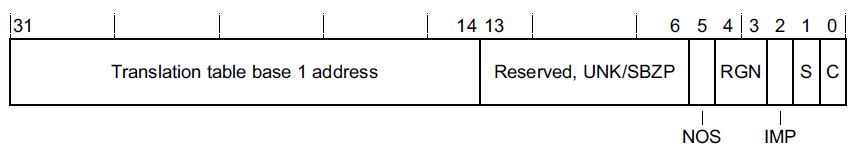
\includegraphics[scale=0.8]{chapters/mmu/figures/ttbr1format}
	\caption{TTBR1 Format \cite[S. B4-1730]{ARM:ARM}}
	\label{fig:TTBR1Format}
\end{figure}

Das Beschreiben der Seitentabellenregister erfolgt, wie bei nahezu jeder MMU-Funktionalität, mittels Assemblerbefehlen, die auf die CP15 Coprozessor Register zugreifen.\\

Beim Füllen der Seitentabellen sind vorgegebene Formate für die beiden Typen von Deskriptoren unbedingt zu beachten. Die Abbildungen \ref{fig:firstLevelDescriptor} und \ref{fig:secondLevelDescriptor} fassen die Formate für first-level und second-level Deskriptoren zusammen. Beiden Deskriptortypen gleich ist die vorgeschriebene Länge von 32 Bit.\\

\subsubsection*{First-level Deskriptoren}

Die First-Level Deskriptortypen werden auf folgende Weise verwendet:

\begin{itemize}
	\item sections für die \ac{MPT} (siehe Abschnitt \ref{subsect:memoryMapping}) 
	\item page table für L1-Seitentabellen von Prozessen (siehe Abschnitt \ref{subsect:memoryMapping})
\end{itemize}

Für die Erstellung von first-level Deskriptoren wurde eine Struktur erstellt, welche in Listing \ref{codeFirstLevelDescriptor} aufgeführt ist. Diese Struktur und jene des second-level Deskriptors wird bei den nachfolgenden Erläuterungen zur MMU benötigt.\\

\begin{figure}[H]
	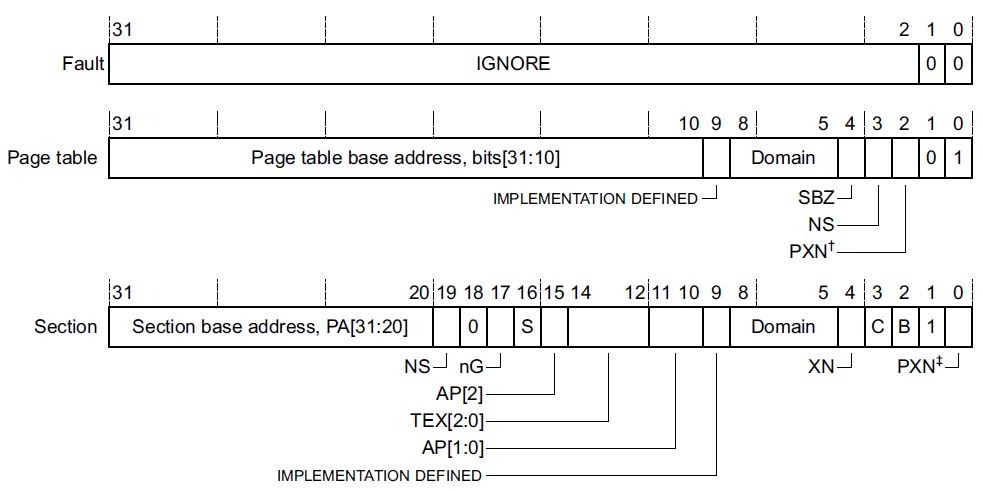
\includegraphics[scale=0.7]{chapters/mmu/figures/firstLevelDescriptor}
	\caption{First-Level Deskriptorformate \cite[S. B3-1326]{ARM:ARM}}
	\label{fig:firstLevelDescriptor}
\end{figure}


\lstinputlisting[language=C, caption=Struktur für first-level Deskriptoren, captionpos=b, label=codeFirstLevelDescriptor]{chapters/mmu/codefiles/firstLevelDescriptor.c}

\subsection*{Second-level Deskriptoren}

In der Speicherverwaltung des Betriebssystems werden ausschließlich small pages verwendet. Ausschlaggebende Gründe, warum small pages den Vorzug gegenüber large pages erhielten, sind die folgenden:

\begin{itemize}
	\item small pages müssen nur einmal in die L2-Seitentabelle eingetragen werden, large pages hingegen 16 mal
	\item L1- und L2-Seitentabellen, die 16 kB bzw. 1 kB Speicher benötigen, belegen bei ihrer Erzeugung nur vier volle page frames bzw. ein page frame physikalischen Speichers zu einem Viertel. Dadurch wird die Speicherfragmentierung verglichen mit large pages stark verringert
\end{itemize}

Die Zusammensetzung der Struktur für second-level Deskriptoren ist in Listing \ref{codeSecondLevelDescriptor} dargestellt.\\

\begin{figure}[H]
	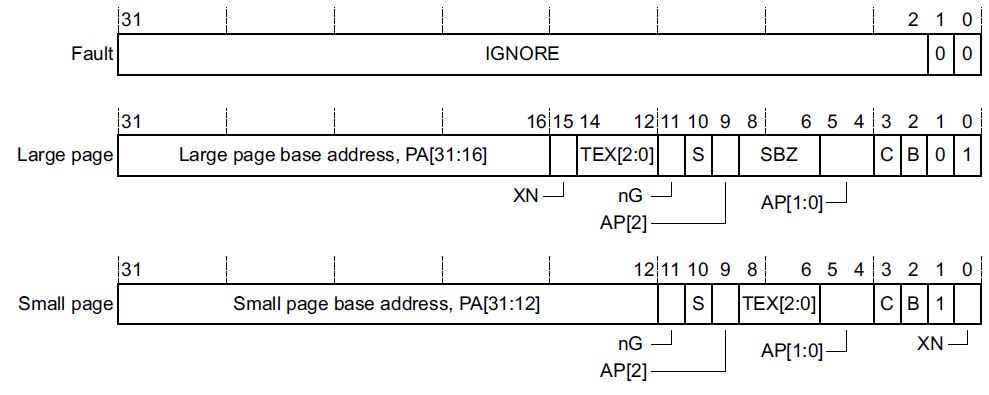
\includegraphics[scale=0.7]{chapters/mmu/figures/secondLevelDescriptor}
	\caption{Second-Level Deskriptorformate \cite[S. B3-1327]{ARM:ARM}}
	\label{fig:secondLevelDescriptor}
\end{figure}


\lstinputlisting[language=C, caption=Struktur für second-level Deskriptoren, captionpos=b, label=codeSecondLevelDescriptor]{chapters/mmu/codefiles/secondLevelDescriptor.c}


\subsection{Aufteilung des virtuellen Speichers und Mapping}
\label{subsect:memoryMapping}

Die Speicherverwaltung des Betriebssystems kann Abbildung \ref{fig:MemoryMap} entnommen werden. Die rechte Seite stellt das physikalische Speichermapping dar und wurde dem Datenblatt des ARM \cite[S. 155]{ARM:TRM} entnommen. Die linke Seite zeigt die Aufteilung des virtuellen Speichers.\\

Organisiert ist der virtuelle Speicher in Speicherregionen. Eine zusätzliche Aufteilung betrifft die Zuständigkeitsbereiche für die Seitentabellenregister TTBR0 und TTBR1. Der ARM Cortex-A8 bietet die Möglichkeit, den virtuellen Speicher in einen \emph{Prozessbereich} und einen \emph{Kernelbereich} aufzuteilen. Der Prozessbereich enthält dabei alle virtuellen Adressen, die für Prozesse zugänglich sind. Der Kernelbereich enthält Komponenten, die sich bei Prozesswechseln nicht ändern. Dazu zählen das Betriebssystem selbst sowie die memory-mapped I/O. \\ 

Die Einstellungen zur Aufteilung des virtuellen Speichers werden im  TTBCR (Translation Table Base Control Register) vorgenommen. Die möglichen Aufteilungsbereiche finden sich in Tabelle B3-1, \cite[S. B3-1330]{ARM:ARM}.\\

Physikalisch steht 1 GB Speicher für die page frames zur Verfügung. Dieser wird im virtuellen Speicher an die Adressen 0x00000000 bis 0x3FFFFFFF gemapped. Die Komponenten der Kernelregion, die sich bei Prozesswechseln nicht ändern, beginnen bei Adressen ab 0x40000000. Damit ergibt sich eine Aufteilung des virtuellen Speichers, wie sie in Abbildung \ref{fig:MemoryMap} dargestellt ist, mit der Bereichsgrenze 0x40000000.\\

Die Adressen ab der Bereichsgrenze bis zu den vollen 4 GB virtuellem Speicher bei der Adresse 0xFFFFFFFF werden in eine so genannte L1 \ac{MPT} gemapped. Bei der Aktivierung der MMU wird die Adresse dieser master page table in das Register TTBR1 geschrieben. Danach wird TTBR1 während der Laufzeit des Betriebssystems nicht mehr verändert.\\

Bei der Initialisierung eines Prozesses wird für den Prozess eine L1 page, die den Prozessbereich abdeckt, angelegt. Soll ein Prozess zur Ausführung gebracht werden, muss seine L1 page table in das TTBR0 geschrieben werden. Das TTBR0 muss zur Laufzeit des Betriebssystems bei Kontextwechseln von Prozessen aktualisiert werden.\\


\begin{figure}[H]
	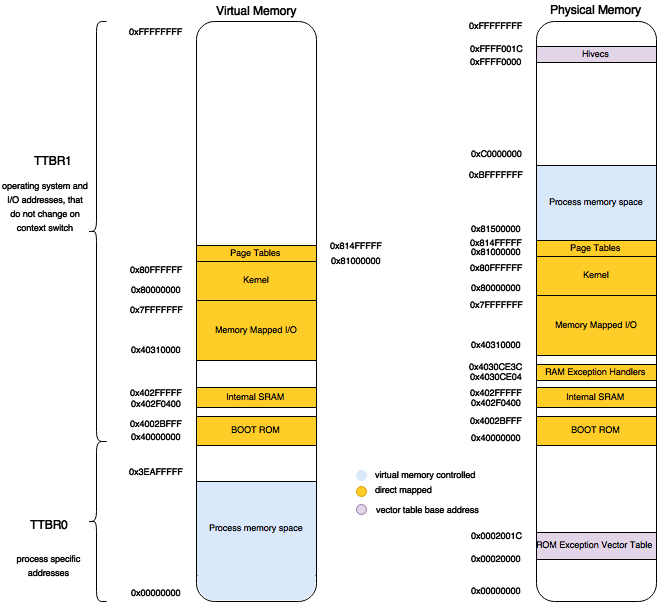
\includegraphics[scale=0.60]{chapters/mmu/figures/MemoryMap}
	\caption{Memory Map des Betriebssystems}
	\label{fig:MemoryMap}
\end{figure}




\begin{table}[H]
\begin{tabular}{p{7cm} | p{7cm}}
  \textbf{Eigenschaft} & \textbf{Beschreibung} \\ \hline
  Größe der Pages & 4 kB\\
  Virtueller Speicher für Prozesse & 1003 MB\\
  Max. Anzahl von L1 und L2 Page Tables & 320 L1 Page Tables oder 1 L1 Page Table + 1276 L2 Page  Table\\
  Theoretisch Max. Anzahl von Prozessen & 320\\
 \end{tabular}
 \caption{Eigenschaften der virtuellen Speicherverwaltung des OS}
 \label{table:SpecifiedVirtualMemory}
\end{table}

\subsubsection{Speicherregionen}

Das nachfolgende Listing \ref{codeMemoryRegion} zeigt die Struktur, mit welcher Regionen im virtuellen Speicher erstellt und verwaltet werden. Sie bieten die Möglichkeit, unterschiedlich große Bereiche des virtuellen Speichers mit denselben Eigenschaften und Zugriffsrechten zu versehen.\\

Erstellt werden solche Speicherregionen sämtliche in Abbildung \ref{fig:MemoryMap} gezeigten Bereiche. Sie enthalten die virtuelle Anfangs- und Endadresse der Region sowie Pagegröße und Zugriffsrechte auf die Region. Weiters enthalten sie eine verkettete Liste von Strukturen, die den Status(reserviert oder nicht reserviert) der einzelnen Pages verwaltet.\\

\lstinputlisting[language=C, caption=Struktur für die Verwaltung von Speicherregionen, captionpos=b, label=codeMemoryRegion]{chapters/mmu/codefiles/region.c}
\vspace{0.5cm}

Zusammengefasst dargestellt sind in Tabelle \ref{table:MemoryRegions} alle Speicherregionen des Betriebssystems. Ein direktes Mapping bedeutet dabei, dass die virtuelle Adresse der physikalischen entspricht.\\

\begin{table}[H]
\begin{tabular}{p{4cm} | p{1.5cm} | p{1.5cm} | p{6cm}}
  \textbf{Region} & \textbf{Mapping} & \textbf{Größe} & \textbf{Beschreibung} \\ \hline
  Page Tables & direkt & 5 MB & Speicherort für L1 und L2 page tables\\
  Kernel & direkt & 16 MB & Speicherort für das Betriebssystem\\
  Memory-Mapped I/O & direkt &  1 GB & Peripheriemodule\\
  Exception Handlers & direkt &  4 kB & Enthält die Exception vector table\\
  Internal SRAM & direkt & 64 kB & Enthält die Exception handler\\
  BOOT ROM & direkt & 192 kB & für zukünftige Erweiterungen \\ 
  Process memory space & virtuell & 1 GB & Speicherbereich für Prozesse
 \end{tabular}
 \caption{Angelegte Speicherregionen}
 \label{table:MemoryRegions}
\end{table}


\subsubsection{Master Page Table}

Um das Mapping der \ac{MPT} verstehen zu können, wird nochmals auf den Adresstranslationsablauf in Abbildung \ref{fig:sectionTranslation} verwiesen. Alle direkt gemappten Regions aus Tabelle \ref{table:MemoryRegions} werden in die L1 \ac{MPT} als 1 MB Sections gemapped.\\

Die Adresse eines Eintrags in der page table setzt sich zusammen aus der Basisadresse der entspreche page table und einem Index. Nach dem setzen der Attribute des page table Eintrags wird durch die Funktion \emph{mmuGetTableIndex} aus den obersten Bits der physikalischen Adresse der Intex in der page table berechnet. Der Index muss um 2 bit nach links geshiftet werden, um das Alignment von 4 Byte einzuhalten. Schließlich wird der geshiftete Index noch durch die Datentypgröße von 4 Byte geteilt. Damit wird die korrekte Adresse des zu schreibenden Tabelleneintrags durch Pointerarithmetik ermittelt. An diese Adresse wird nun der Eintrag geschrieben, der zuvor durch die Funktion \emph{mmuCreateL1PageTableEntry} aus der übergebenen first-level Deskriptorstruktur erstellt wurde. Listing \ref{codeMasterPageTableMapping} zeigt die praktische Ausführung des direkten Mappings in die \ac{MPT}.\\ 


\lstinputlisting[language=C, caption=Funktion für direktes Mapping in die master page table, captionpos=b, label=codeMasterPageTableMapping]{chapters/mmu/codefiles/directMapIntoMasterPageTable.c}

\subsection{Allokierung der Page Frames}

Für die Verwaltung der page frames wurde eine Bitsmap verwendet. Abbildung \ref{fig:BitsMap} zeigt das Prinzip.
Die Bitsmap wird durch ein Array der Länge N/8 Bytes realisiert. N steht hier für die Anzahl der page frames. Das i-te Bit im n-ten Byte der Bitsmap definiert den Verwendungsstatus des (n*8 + i) –ten page frame.




\begin{figure}[H]
	\centering
	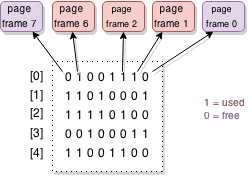
\includegraphics[scale=1]{chapters/mmu/figures/BitsMap}
	\caption{Beispiel einer Bitsmap zur Verwaltung der Page Frames}
	\label{fig:BitsMap}
\end{figure}

\subsubsection{Allokation von Page Frames bei Data Abort Exception}


\begin{figure}[H]
	\centering
	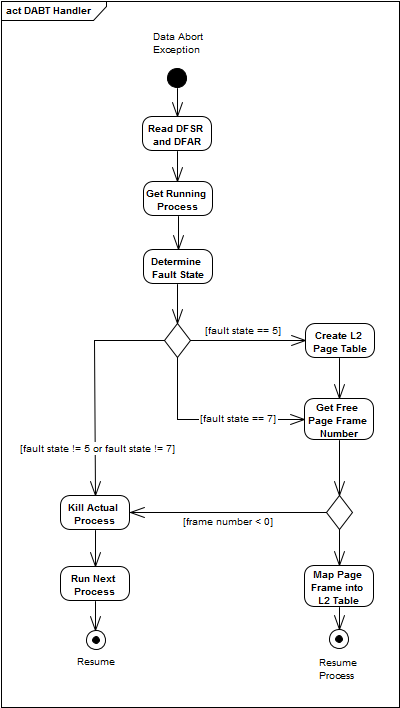
\includegraphics[scale=0.7]{chapters/mmu/figures/DABTHandler}
	\caption{Einlagerung von page frames duch den DABT-Handler}
	\label{fig:dabthandler}
\end{figure}


\subsection{Aktivieren der MMU}
\label{subsect:activateMMU}

Bevor die MMU erfolgreich aktiviert werden kann, muss vorher eine Reihe von Einstellungen gesetzt werden.\\


Listing \ref{codeMMUInit} zeigt den kompletten Ablauf zur Aktivierung der MMU.

\lstinputlisting[language=C, caption=Aktivierung der MMU, captionpos=b, label=codeMMUInit]{chapters/mmu/codefiles/MMUInit.c}


\subsection{Interaktion der MMU mit Prozessen}

Die Schnittstelle der Softwareimplementierung der MMU zeigt Listing \ref{codeMMUFunctions}.\\

\lstinputlisting[language=C, caption=Softwareschnittstelle der MMU, captionpos=b,  label=codeMMUFunctions]{chapters/mmu/codefiles/MMUFunctions.c}
\vspace{0.5cm}

Die Schnittstellenfunktionen werden auf die folgende Weise verwendet: 

\begin{description}
	\item[MMUInit] \hfill \\ Initialisiert die Regionen des virtuellen Speichers und die MMU für die Verwendung. Nach dem Ausführen dieser Funktion ist die MMU eingeschaltet. Bei nach erfolgreichem Ausführen wird als Rückgabewert 1 zurückgeliefert. Diese Funktion wird bei der Initialisierung des Prozess Managers aufgerufen.
	\item[MMUSwitchToProcess] \hfill \\ Bringt den als Parameter übergebenen Prozess zur Ausführung. Dabei wird der TLB geflusht und die Adresse der L1 page table des Prozesses in das TTBR0 geschrieben. 
	\item[MMUInitProcess] \hfill \\ Erstellt beim Erzeugen eines neuen Prozesses eine L1 page table für diesen Prozess. Die page table wird mit fault entries initialisiert.
	\item[MMUHandleDataAbortException] \hfill \\ Diese Funktion wird bei jeder Data Abort Exception ausgeführt. Sie wird durch einen in Assembler implementierten Dabt Handler aufgerufen. Die Funktion lädt die virtuelle Adresse, bei deren Zugriff die Data Abort Exception ausgelöst wurde aus dem \acf{DFAR} sowie den Fehlerstatus aus dem \acf{DFSR}. Die weitere Vorgehensweise wird in Abhängigkeit vom Fehlerstatus durchgeführt.
	\item[MMUFreeAllPageFramesOfProcess] \hfill \\ Beim Killen eines Prozesses gibt diese Funktion sämtliche von diesem Prozess belegten page frames in der zur Verwaltung der page frames eingesetzten Bitsmap wieder frei.
\end{description}

\pagebreak 
\section{Interprozesskommunikation}
Interprozesskommunikation dient zur Kommunikation zwischen verschiedenen Prozessen. Dabei ist entscheidend, dass beiden zu kommunizierenden Prozesse in unterschiedlichen Speicherbereichen bzw. in strikt voneinander getrennten Speicherbereichen sind. 

\subsection{Aufbau}
bla

\subsection{IpcManager}
Der IpcManager händelt die Interprozesskommunikation zwischen Prozessen. Listening \ref{ipcManagerInterface} zeigt die Schnittstelle des Managers.

\lstinputlisting[language=C, caption=Schnittstelle des IpcManagers, captionpos=b,  label=ipcManagerInterface]{chapters/ipc/codefiles/ipcmanager-interface.c}

\pagebreak 
\section{Treiber}
Die Treiber stellen eine abstrakte Schnittstelle auf den Hardware Abstraction Layer dar. Dadurch muss nicht mehr direkt auf die einzelnen Hardwarekomponenten zugegriffen werden. Ein wesentlicher Aspekt bei der Architektur der Treiber war Abstraktion. Dadurch wird gewährleistet, dass jeder Treiber über die selbe Schnittstelle angesprochen werden kann. Zudem ist die Verwaltung durch den Driver Manager erleichtert.

\subsection{Aufbau eines Treibers}
In Listening \ref{generalDriverInterface} ist die allgemeine Schnittstelle für jeden Treiber ersichtlich. Jeder implementierte Treiber muss diese vorweisen können, ein Beispiel (LED Treiber) dazu ist in Listening \ref{ledDriver} zu sehen.

\lstinputlisting[language=C, caption=Allgemeine Schnittstelle für einen Treiber, label=generalDriverInterface]{chapters/driver/codefiles/generalDriverInterface.c}

\lstinputlisting[language=C, caption=Implementierung der allgemeinen Treiberschnittstelle (LED Beispiel), label=ledDriver]{chapters/driver/codefiles/ledDriver.c}


\pagebreak 
\section{System API}
Die System API dient als Schnittstelle zum Benutzer bzw. zur Benutzerin. Dabei ist eine saubere Trennung zwischen BenutzerInnen Schnittstelle und Betriebssystem zwingend notwendig.

\subsection{Aufbau eines Systemcall Datenpakets}
Jedem Systemcall werden Daten mitgegeben, dieses müssen zuvor in eine geeignete Datenstruktur transformiert werden. In Listing \ref{systemcall-datapackage} ist die gewählte Datenstruktur abgebildet.


\lstinputlisting[language=C, caption=Aufbau eines Systemcall Datenpakets, captionpos=b, label=systemcall-datapackage]{chapters/systemapi/codefiles/datapackage.c}

\subsection{Vorgehensweise bei einem Systemcall}
Das Vorgehen bei einem Systemcall ist in Abbildung \ref{fig:Sequencediagram-systemcall} ersichtlich. 

\begin{figure}[H]
	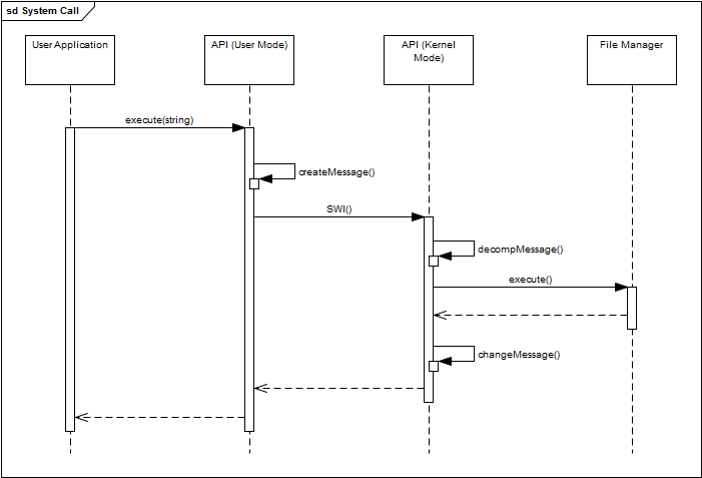
\includegraphics[scale=0.70]{chapters/systemapi/figures/systemcall-sequence-diagram}
	\caption{Sequenzdiagramm eines Systemcalls}
	\label{fig:Sequencediagram-systemcall}
\end{figure}

\pagebreak 
\section{BenutzerInnen-Anwendung}

Bei der BenutzerInnen-Anwendung handelt es sich um die Ansteuerung eines Moving Heads mittels  Digital Multiplex (DMX) Protokoll.  

\subsection{Grundlegender Aufbau des DMX Protokolls}
Es gibt mehrere verschiedene Spezifikationen für das DMX Protokoll. Im folgenden wird eine dieser unterschiedlichen Spezifikation erläutert und anschließend zu Vergleichszwecken verwendet. Abbildung \ref{fig:DMX-512-Protocol} dient zur Veranschaulichung des DMX-512 Protokolls. 

% http://mc.mikrocontroller.com/de/dmx512.php
% TODO: add reference to this webside

\begin{figure}[H]
	
\includegraphics[scale=0.60]{chapters/userapplication/figures/todo}
	\caption{DMX Protokoll}
	\label{fig:DMX-512-Protocol}
\end{figure}

Tabelle \ref{table:DMX-512-Protocol} beschreibt die einzeln nummerierten Markierungen aus Abbildung \ref{fig:DMX-512-Protocol}.

\begin{table}[H]
\begin{tabular}{p{1.5cm} | p{6.5cm} | p{1cm} | p{1cm} | p{1cm} | p{1cm}}
  \textbf{Nummer} & \textbf{Signalname} & \textbf{Min.} & \textbf{Typ.} & \textbf{Max.} & \textbf{Einheit} \\ 
  \hline
  1 & Reset & 88.0 & 88.0 & - & $\mu$s \\
  2 & Mark zwischen Reset- und Startbyte & 8.0 & - & 1 s & $\mu$s \\
  3 & Frame-Zeit & 43.12 & 44.0 & 44.48 & $\mu$s \\
  4 & Startbit & 3.92 & 4.0 & 4.08 & $\mu$s \\
  5 & LSB (niederwertigstes Datenbit) & 3.92 & 4.0 & 4.08 & $\mu$s \\
  6 & MSB (höchstwertigstes Datenbit) & 3.92 & 4.0 & 4.08 & $\mu$s \\
  7 & Stopbit & 3.92 & 4.0 & 4.08 & $\mu$s \\
  8 & Mark zwischen Frames (Interdigit) & 0 & 0 & 1.0 & s \\
  9 & Mark zwischen Paketen & 0 & 0 & 1.0 & s \\
  - & Reset-Reset (Paketabstand) & 1094 & - & - & $\mu$s \\
 \end{tabular}
 \caption{Eigenschaften des DMX-512-Protokolls}
 \label{table:DMX-512-Protocol}
\end{table}

Die Übertragungsgeschwindigkeit ist bei allen Protokollarten identisch und beträgt 250 kBaud, d.h. jedes Bit hat eine Dauer von 4 $\mu$ s. Das DMX Protokoll besitzt 512 verschiedene Kanäle, wobei jeder Kanal mithilfe eines Datenbytes gesteuert wird. In Abbildung \ref{fig:DMX-512-Protocol} ist ersichtlich, dass jedes übertragene Datenbyte zusätzlich ein Startbit sowie zwei Stopbits besitzt. Somit ergeben sich für jeden Kanal genau elf Bits.

\subsection{Messergebnisse des Implementierten DMX Protokolls}

\begin{figure}[H]
	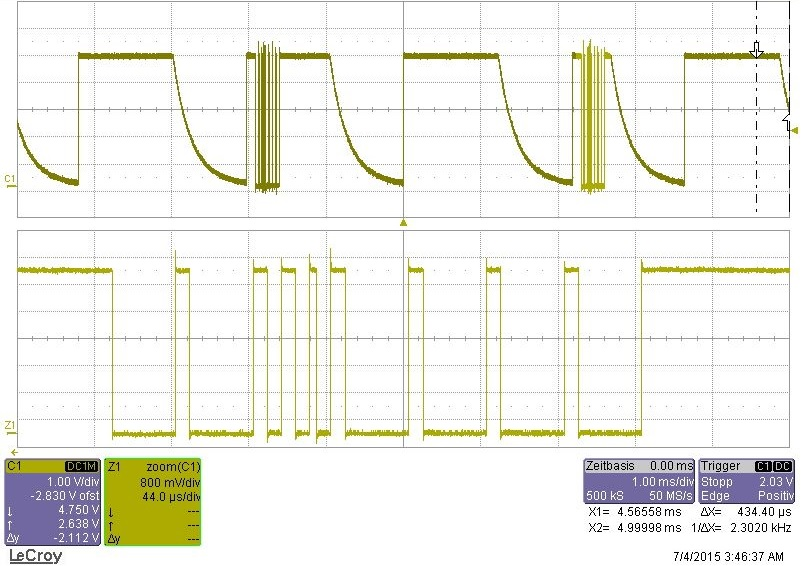
\includegraphics[scale=0.7]{chapters/userapplication/figures/DMX-Edge}
	\caption{DMX Protokoll: Problem fallende Flanke}
	\label{fig:DMX-Edge}
\end{figure}

\begin{figure}[H]
	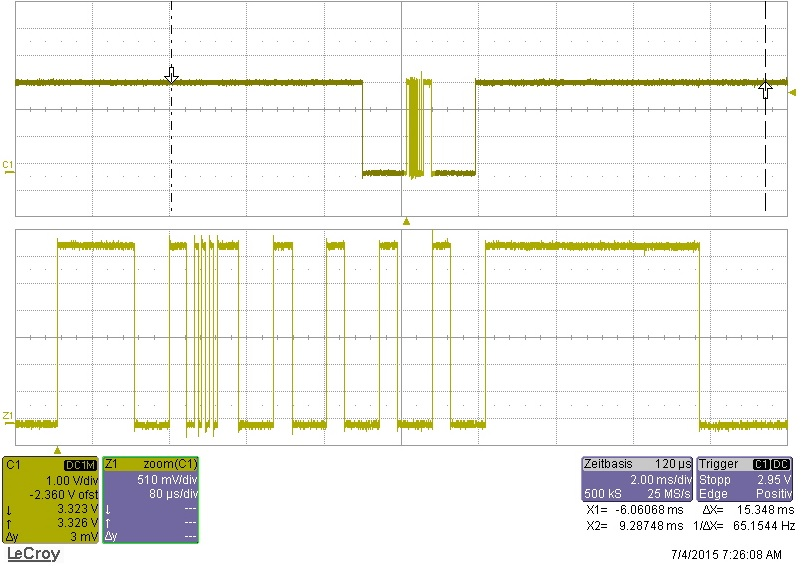
\includegraphics[scale=0.7]{chapters/userapplication/figures/DMX-Offset-Byte}
	\caption{DMX Protokoll: Problem Offset Byte}
	\label{fig:DMX-Offset-Byte}
\end{figure}

\begin{figure}[H]
	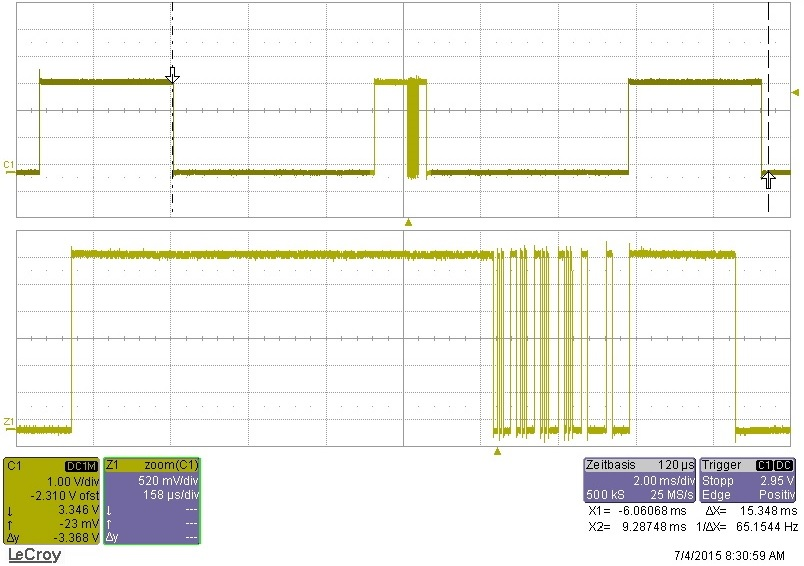
\includegraphics[scale=0.7]{chapters/userapplication/figures/DMX}
	\caption{Funktionierendes DMX Protokoll}
	\label{fig:DMX}
\end{figure}

\pagebreak 
\section{Performanzuntersuchungen}
\label{Performanz}

In diesem Kapitel werden Performanzeaspekte des Betriebssystems dokumentiert und diskutiert. Die Performanz des Betriebssystems wurde mittels verschiedener Experimente und Messungen untersucht, deren Resultate im Folgenden beschrieben sind.

\subsection{Messung und Ergebnisse}
Um die Performanz des Betriebssystems beurteilen zu können, wurden zeitliche Messungen der relevanten Unterbrechungen vorgenommen. Die Messungen der einzelnen Unterbrechungen wurden mit Hilfe eines Oszilloskops durchgeführt, wobei alle Messungen jeweils zehn mal vorgenommen wurden und schließlich der Durchschnitt über alle Messungen als Resultat herangezogen wurden. In Tabelle \ref{table:osciResults} sind die einzelnen Messungen und Resultate aufgelistet.

\begin{table}[H]
\begin{tabular}{p{7cm} | p{7cm}}
  \textbf{Testfall} & \textbf{Durchschnittszeit ($n=10$)} \\ \hline
  	\ac{MMU} Fault State 5 & $~18.90 ms$ \\
  	\ac{MMU} Fault State 7 & $~11.80 ms$ \\
  	\ac{MMU} Freeing Page Frame & $~19.80 ms$ \\
  	Zeitscheibe (effektiv) & $~10.04 ms$ \\
  	\textit{Context Switch} & $~375 \mu s$ \\
 \end{tabular}
 \caption{Performanz-Messergebnisse}
 \label{table:osciResults}
\end{table}

Interessant ist vor allem die vergleichsweise lange Unterbrechung eines \textit{Context Switch}, welcher knapp $3\%$ der gesamten Zeitscheibe eines Prozesses in Anspruch nimmt. In Anbetracht dieser Messergebnisse wäre für die Gesamtperformanz des Betriebssystems durchaus zu überlegen, entweder die Zeitscheibe eines Prozesses zu verlängern oder aber die Logik für den \textit{Context Switch} zu optimieren.\\
Von Interesse sind auch die beiden Fälle der Einlagerung eines \textit{Page Frame}. \ac{MMU} \emph{Fault State 5} stellt dabei den Fall der Erstellung einer \textit{Level 2 Page Table} samt Einlagerung eines \textit{Page Frame} dar, \ac{MMU} \emph{Fault State 7} stellt dagegen lediglich die bloße Einlagerung eines \textit{Page Frame} in eine \textit{Level 2 Page Table} dar. Nachdem diese Unterbrechungen vergleichsweise selten auftreten, sind hier Optimierungen nicht unbedingt hochprior anzunehmen.

\pagebreak 
\section{Zusammenfassung und Ausblick}
\label{summary}

In diesem Kapitel werden die erreichten Ergebnisse zusammengefasst. Weiters wird ein Ausblick auf Möglichkeiten der Weiterentwicklung geboten.

\subsection{Zusammenfassung}

Das primäre Ziel dieses Projektes war die Erlangung tiefergehende Kenntnisse in Bezug auf die Systemprogrammierung von Systemen mit beschränkten Ressourcen. Dabei sollten vor allem die theoretische Grundlagen von Betriebssystemen praktisch umgesetzt werden. \\
 
Implementiert und getestet wurde ein Betriebssystem welches sich auch in Langzeittests als stabil erwiesen hat. Das Betriebssystem ist durch die HAL flexibel und ohne größere Aufwände protierbar. Zudem ist es möglich, von einer MicroSD-Karte Applikationen zu laden und auszuführen. 
Bei der Implementierung wurden sämtliche Grundaspekte moderner Betriebssysteme, wie beispielsweise die Interprozesskommunikation oder die virtuelle Speicherverwaltung, behandelt. Zudem wurden die Sicherheitsrisiken durch das saubere Trennen der Adressräume und Benutzermodi stark verringert. \\
 
Es ist zu erwähnen, dass während des Entwicklungsprozesses erwartete wie auch nichterwartete Probleme aufgetreten sind. Diese betreffen in erster Linie Komplikationen, die durch falsches Setzen der Hardwareregister entstanden sind. \\
 
Für das entworfene Betriebssystem wird kein Anspruch auf Vollständigkeit erhoben, da seine Entwicklung agil vorgenommen wurde. So wurden aus Zeitgründen bei der Erstellung der HAL nur die für die vorgesehene DMX-Applikation benötigten Funktionen implementiert. \\
 

\subsection{Ausblick}

Das Betriebssystem ist in der vorliegenden Form voll einsatzbereit und erfüllt alle gesetzten Anforderungen. Daher wird an dieser Stelle seine Entwicklung seitens des Projektteams eingestellt. Unter dem in der Einleitung angegebenen Repository auf GitHub kann es frei zugänglich heruntergeladen werden. Nachfolgend werden Ansatzpunkte für Verbesserungen bzw. Weiterentwicklungen augelistet.

\subsubsection{Punkte mit Verbesserungspotential}
Einige Punkte des Betriebssystem konnten nicht vollständig abgedeckt werden. Diese Punkte mit Verbesserungspotential werden in Tabelle \ref{table:points-to-improve} kurz beschrieben.

\begin{table}[H]
\begin{tabular}{p{5cm} | p{9cm}}
  \textbf{Sachverhalt} & \textbf{Beschreibung}
  \\ \hline
  Caching & Die aktuelle Speicherverwaltung ist ein non-caching System. Eine Einführung des Cachings für Daten hätte eine Verbesserung der Performance zur Folge. \\
  
 \end{tabular}
 \caption{Übersicht der Punkte mit Verbesserungspotential}
 \label{table:points-to-improve}
\end{table}

\subsubsection{Fehlende Punkte für eine praktische Verwendung des Betriebssystems}
Das Betriebssystem weist einige wenige Punkte auf, welche noch nicht implementiert wurden, aber für eine praktische Verwendung fehlen. Tabelle \ref{table:missing-points} zeigt diese Punkte auf.

\begin{table}[H]
\begin{tabular}{p{5cm} | p{9cm}}
  \textbf{Fehlender Punkt} & \textbf{Beschreibung}
  \\ \hline
  ResourceManager & Dieser Manager ist für die Verwaltung von Ressourcen zuständig. Dazu zählen XXX\\
  
 \end{tabular}
 \caption{Übersicht der fehlenden Punkte}
 \label{table:missing-points}
\end{table}
\section{Ausblick}
Diese Kapitel enthält befasst sich mit Inhalten, welche in diesem Betriebssystem nicht zur Gänze implementiert wurden bzw. noch Verbesserungspotential aufweisen.

\subsection{Offene Punkte aus den Anforderungen}
Das Betriebssystem schneidet alle Punkte, welche in den Anforderungen erwähnt wurden, zumindest teilweise an.

\subsection{Punkte mit Verbesserungspotential}
Einige Punkte des Betriebssystem konnten nicht vollständig abgedeckt werden. Diese Punkte mit Verbesserungspotential werden in Tabelle \ref{table:points-to-improve} erläutert.

\begin{table}[H]
\begin{tabular}{p{5cm} | p{9cm}}
  \textbf{Punkt mit Potential} & \textbf{Beschreibung}
  \\ \hline
  XXX & XXX \\
  
 \end{tabular}
 \caption{Übersicht der Punkte mit Verbesserungspotential}
 \label{table:points-to-improve}
\end{table}

\subsection{Fehlende Punkte für eine praktische Verwendung des Betriebssystems}
Das Betriebssystem weist einige wenige Punkte auf, welche noch nicht implementiert wurden, aber für eine praktische Verwendung fehlen. Tabelle \ref{table:missing-points} zeigt diese Punkte auf.

\begin{table}[H]
\begin{tabular}{p{5cm} | p{9cm}}
  \textbf{Fehlender Punkt} & \textbf{Beschreibung}
  \\ \hline
  ResourceManager & Dieser Manager ist für die Verwaltung von Ressourcen zuständig. Dazu zählen XXX\\
  
 \end{tabular}
 \caption{Übersicht der fehlenden Punkte}
 \label{table:missing-points}
\end{table}

\pagebreak 

\clearpage
\phantomsection
\addcontentsline{toc}{chapter}{Literaturverzeichnis}
\bibliography{./bib/Bibliography}

\end{document}